\scanpage{8}
chosen --- if one \deleted{multiplies} replaces $g$ by $\operatorname{int}(\lambda)u$ with $\lambda=l_0^\alpha\in L_0$ ($\alpha\in\hat{\mathbb Z}^{*}$), then $g$ is replaced by
\[
\lambda g\rho(\unsure{l_0|\lambda})^{-1}=\uline{l_0^\alpha gl_1^{-\alpha}}.
\]
This being so, \deleted{\unsure{the|the}} the relations $(*)$ and $(**)$ determine $u$ in terms $p\in\hat{\mathbb Z}^{*}$ and of $g\in\unsure{\pi|\Pi}$, by
\[
\left\{\begin{aligned}
u(l_0)&=l_0^p\\
u(l_1)&=u\rho(l_0)=\operatorname{int}(g)\rho\underbrace{u(l_0)}_{l_0^p}=\operatorname{int}(g)l_1^p\\
u(l_\infty)&=u\rho(l_1)=\operatorname{int}(g)\rho\underbrace{u(l_1)}_{\operatorname{int}(g)l_1^p}\\
&=\operatorname{int}(g)\underbrace{\rho\operatorname{int}(g)\rho^{-1}}_{\unsure{\operatorname{int}(\rho(g))}}\underbrace{(\rho l_1^p)}_{l_\infty^p}
=\deleted{\unsure{\operatorname{int}(g\rho(g))l_\infty^p|\operatorname{int}g\rho(g)l_\infty^p|\operatorname{int}(g\rho(g))l_\infty}}\inserted{\operatorname{int}g\rho(g))l_\infty^p}
\end{aligned}\right.
\]
\margin{\uline{NB} We see that \unsure{$u$|$g$|$u_g$} automatically respects the structure with loops, with the multiplier $p$}

One must check, to indeed have an endomorphism of $\pi$, \uline{the relation $l_0'l_1'l_\infty'=1$} i.e.
\figure{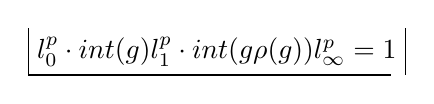
\begin{tikzpicture}[baseline=(m.base)]\node[inner sep=3pt] (m) {$l_0^p\cdot\operatorname{int}(g)l_1^p\cdot\operatorname{int}(g\rho(g))l_\infty^p=1$};\draw (m.north west)--(m.south west)--([xshift=-.18cm]m.south east);\draw (m.north east)--(m.south east);\end{tikzpicture}}
or again
\[
l_0^p(gl_1^pg^{-1})(g\rho(g)l_\infty^p\rho(g)^{-1}g^{-1})=1
\]
i.e.
\[
l_0^pgl_1^p\rho(g)l_\infty^p\rho(g)^{-1}g^{-1}=1
\]
or again, moving the $g^{-1}$ to the left
\[
\deleted{l_0^p\cdot\operatorname{int}(g)\bigl(l_1^p\cdot\operatorname{int}(\rho(g))(l_\infty^p)\bigr)=1}
\]
\[
\operatorname{int}g^{-1})l_0^p\cdot l_1^p\cdot\operatorname{int}(\rho(g)(l_\infty^p)=1
\]
The relations $\unsure{(*)2|(*)_2|(*),}$ and $(**)$ are satisfied by construction (for $**$, it suffices $\bar m$ to check it for the value on both sides at $l_0\ l_1$).
\mspage{7}
